\TOWRITE{ALL}{Proofread WP 1 Management pass 1}
\begin{draft}
\TOWRITE{PS (Work Package Lead)}{For WP leaders, please check the following (remove items
once completed)}
\begin{verbatim}
- [ ] have all the tasks in this Work Package a lead institution?
- [ ] have all deliverables in the WP a lead institution?
- [ ] do all tasks list all sites involved in them?
- [ ] does the table of sites and their PM efforts match lists of sites for each task?
      (each site from the table is listed in all relevant tasks, and no site is listed
      only in the table or only at some task)
\end{verbatim}
\end{draft}

\begin{workpackage}[id=core,wphases=0-48,swsites,
  title=Structural improvements to Jupyter,
  short=Core,
  lead=SRL,
  % EGIRM=4,
  % INSERMRM=4,
  QSRM=15,
  % SILRM=4,
  SRLRM=30,
  % UIORM=4,
  UPSUDRM=14,
  WTTRM=8,
  XFELRM=16,
  EPRM=13,
]
\begin{wpobjectives}
  \begin{compactitem}
    \item to support and maintain core Jupyter infrastructure in order to keep it healthy
         and useful for open science
    \item to develop new features in the core of Jupyter to bring it to a wider community
    \item to develop new features in the core of Jupyter to make it more effective
         in facilitating open science

 \end{compactitem}
\end{wpobjectives}

\begin{wpdescription}

Community-led open source software is critical to a sustainable future for open science.
Commonly used tools make up a shared infrastructure,
where investment in core components benefits the widest user community.
\TheProject is centred around the Jupyter project,
which is a collection of projects for interactive computing and
communicating computational ideas.

This work package is focused on developing and maintaining
the core of Jupyter.
In particular, we will help maintain these projects to meet the needs of the
Jupyter community, with a focus on needs for open science.
To serve the needs of \TheProject,
Jupyter core infrastructure will need improvements
to security, performance, and scalability,
which will be provided in \localtaskref{maintenance}.
In addition, we will develop new features in the core of Jupyter
to bring it to a wider audience,
and to improve its usefulness to those working toward open science practices,
including via collaboration features (\localtaskref{collaboration})
and accessibility (\localtaskref{accessibility}).


\end{wpdescription}

\begin{tasklist}

\begin{task}[
  title=Maintenance of Jupyter and JupyterHub,
  id=maintenance,
  lead=SRL,
  PM=44,
  wphases={0-48},
  partners={XFEL,UPSUD,QS}
]

\begin{figure}[ht!]\centering
  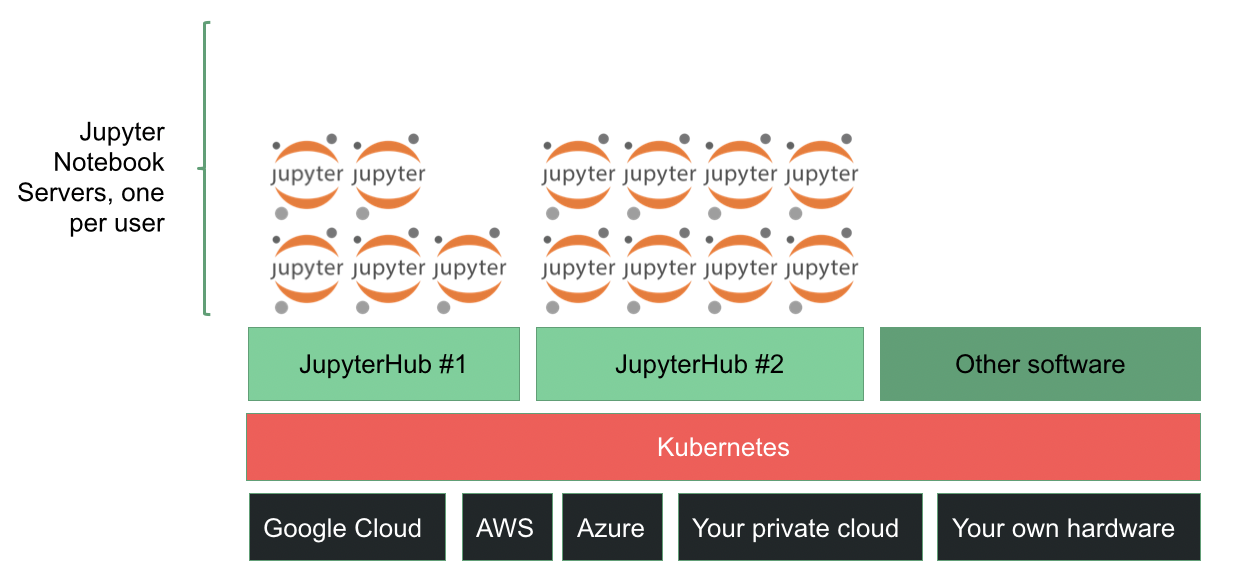
\includegraphics[width=0.6\textwidth]{images/jupyterhub-kube.png}
  \caption{
  Jupyter notebooks deployed for many users
  on shared infrastructure using JupyterHub and Kubernetes.
  }
  \label{fig:jupyterhub-kubernetes}
\end{figure}

  Developing software that people will use requires maintenance of that software,
  not just new development.
  Millions of people rely on Jupyter software,
  including all participants in \TheProject,
  and with this proposal, we fund general support of the Jupyter infrastructure.

  Maintenance of core software is often an implicit and un-paid cost,
  or one hidden in over-describing the resources required to deliver
  proposed developments.
  In \TheProject, we make it clear and explicit that we will spend a significant amount
  of time developing and maintaining the core Jupyter and JupyterHub
  e-Infrastructure to respond to the needs of \TheProject and others,
  and help keep it a healthy and active software community.

  We will contribute to supporting Jupyter e-Infrastructure software,
  ensuring that it meets the needs (\localdelivref{jupyter-contributions})
  of \TheProject,
  and aid in the release process to ensure that stable releases
  of Jupyter software can be used in mature \TheProject services
  (\localdelivref{jupyter-releases}).

  \TheProject will need improvements to core Jupyter functionality, including areas of:

  \begin{compactenum}
    \item ease of deployment
    \item security
    \item scalability of JupyterHub
    \item performance
  \end{compactenum}

  We will contribute improvements in these areas,
  meeting the needs of \TheProject and benefiting the wider Jupyter
  community.

\end{task}

% template for a task
% each task should be added to exactly one workpackage
% in the workpackage task list
\begin{task}[
  title=JupyterHub / BinderHub convergence,
  id=jh-bh-conv,
  lead=EP,
  PM=16, % EP: 12PM, WTT: 2PM, PSUD: 2PM
  wphases={0-36},
  partners={WTT}]

  \textbf{Scenario}

  An institution -- typically a university, a national lab, a transnational
  research infrastructure such as the European XFEL, or transnational
  infrastructure provider like EGI, or even an NGO or SME -- wishes to provide its members and
  users with a Jupyter service.

  The service lets user spawn and access personal or collaborative virtual
  environments: namely a web interface to a light weight virtual machine,
  in which they can use Jupyter notebooks, run calculations, etc.

  To cater for a large variety of use cases in teaching and research,
  the main aim of the upcoming specifications is to make the service as
  versatile as possible. In particular, it should empower the users to 
  customize the service (available software stack, storage setup, ...),
  without a need for administrator intervention.

  \textbf{State of the art}
  JupyterHub already provides authentication, persistent storage and some
  default environments for its users. On the other hand, BinderHub offers
  the possibility to define more precisely the requirements for your teaching
  or research environment which makes it very flexible. However, BinderHub is still missing the  
  authentication and persistent storage capabilities provided by JupyterHub.

  \textbf{This task}
  The purpose of this task is to have the same services offered by JupyterHub
  (authentication, persistent storage, ...) with the flexibility of BinderHub
  (construction of your own environment for teaching or research).

  % Motivation: \TODO{reuse material from the blog post:
  % \url{https://opendreamkit.org/2018/03/15/jupyterhub-binder-convergence/}}
  % \TODO{reuse material from the hackmd notes with Tim:
  % \url{https://hackmd.io/0DLDCXcmRzC_dOwjEak3hg#}}
  The task includes the following activities:
  \begin{compactitem}
  \item Extend where needed JupyterHub's authentication features% (OIDC, ...)
  \item Credential management
  \item Customizable persistence at the admin, and user level
  \item Choice of container registry at the admin and user level % Could be moved to the repo2docker/binder task
  \item Runtime resource configuration % (disk, memory, cpus, time, ...)
  \end{compactitem}
  We will provide a report explaining how to make JupyterHub/Binder convergence a reality (\localdelivref{jh-bh-conv-report}).
\end{task}

\begin{task}[
  title=Accessibility in Jupyter,
  id=accessibility,
  lead=SRL,
  PM=12,
  wphases={12-36!.5},
  partners={}
]

  Improving the accessibility of Jupyter software
  is important to ensuring the value of \TheProject reaches and appropriately supports
  the broadest community.
  In particular, we should take advantage of established guidelines (such as a11y) and
  technologies to ensure that people with visual impairments can make full use
  of the software.
  This includes considerations such as font size and contrast ratios,
  as well as ensuring that the interface can be used with a screen reader,
  for people who cannot use a conventional display screen.

  Working with the community and UI accesibility experts, we will audit the accessibility 
  of Jupyter software and assemble a roadmap for improved accessibility
  (\localdelivref{accessibility-report}),
  and ultimately work to improve the accessibility of Jupyter software,
  starting with JupyterHub (\localdelivref{accessibility}).
\end{task}

% each task should be added to exactly one workpackage
% in the workpackage task list
\begin{task}[
  title=Multi-device Real-time Collaboration,
  id=collaboration,
  lead=UPSUD,
  PM=24,       % UPSUD: 12, XFEL: 2, QS:9, EP: 1
  wphases={0-48},
  partners={QS,XFEL,EP}
]
  % For applications such as real-time collaboration and others,
  % it can be beneficial.
  % We will explore different possible mechanisms for moving document state
  % to the server-side in JupyterLab.

  \TODO{Put into perspective w.r.t. prior art, in ODK and elsewhere}

Collaboration is tremendously important in both research and industry,
so the ability to collectively edit and run notebooks would be invaluable.
It's also increasingly common for each person to use multiple devices to
manipulate or present content, and seamlessly transferring updates between them
presents similar technical challenges.
Jupyter already recognizes the distributed nature of the digital environment by supporting remote kernels for computation,
but the interface assumes that one user at a time works on a notebook from
one device.
BOSSEE will embrace this multi-device world and facilitate the distribution and
real-time collaborative editing of content across multiple devices for presentation, interaction and collaboration purposes.

There are already some services providing real-time collaboration atop
notebooks. Google offers \emph{Colaboratory} \cite{Colab}, a proprietary
web application using its \emph{Google Drive} backend.
\emph{CoCalc} \cite{Cocalc} provides a suite of tools for collaborative
mathematical computing, including an open-source mechanism for real-time
collaboration on notebooks, but this is tightly integrated with that service's
infrastructure.
We want to make realtime collaboration available to as many Jupyter users as
possible, however they choose to install and use the notebook software.

We will create a real-time collaborative notebook or JupyterLab-like application by leveraging well-known synchronization techniques such as Operational Transformation (OT) or Conflict-free Replicated Data Types (CRDTs), with server-side hosting of the document state. 
We will build on our experience with Webstrates (\url{http://webstrates.net}), a web-based environment that supports real-time sharing of web content. The CodeStrates extension to Webstrates uses the layout of Jupyter notebooks, and we have created a proof-of-concept showing that it can work with Jupyter kernels. However CodeStrates, and there are interesting unresolved questions about code execution in such a shared environment: Should it be synchronized or not among participants? Should there be a single kernel or one per participant? etc.

We will also enable selective distribution, aggregation and control of content across devices. 
We have used Webstrates to distribute and synchronize content across multiple devices such as a tablet, a laptop and a large wall-sized display. Yet this does not cover all use cases. 
For example, in a meeting, the participants should each be able to run their own notebook and pick which content to share with the group on a large display. 
We will create an environment where a notebook can collect specific cells from another notebook, or where a JupyterLab widget aggregates data from a collection of widgets running on each user’s device. 
We also want to support remote interaction using one device to control another, e.g. a widget on a smartphone to control a parameter in a computation taking place in a particular notebook, whose result is shown on a large shared display.

  % \begin{compactitem}
  % \item ...
  %   (\localdelivref{deliv-id})
  % \end{compactitem}

\end{task}


\end{tasklist}


\begin{wpdelivs}
  % \begin{wpdeliv}[due=1,miles=startup,id=infrastructure,dissem=PU,nature=DEC,lead=SRL]
  %   {Some Deliverable}
  % \end{wpdeliv}

  \begin{wpdeliv}[due=24,miles=prototype,id=jupyter-contributions,dissem=PU,nature=OTHER,lead=SRL]
    {Contributions to core Jupyter and JupyterHub software}
  \end{wpdeliv}

  \begin{wpdeliv}[due=48,miles=final,id=jupyter-releases,dissem=PU,nature=OTHER,lead=SRL]
    {Public releases of core Jupyter and JupyterHub software supporting \TheProject services}
  \end{wpdeliv}

  \begin{wpdeliv}[due=24,miles=prototype,id=jh-bh-conv-report,dissem=PU,nature=R,lead=EP]
    {Guidelines for a JupyterHub/Binder convergence}
  \end{wpdeliv}

  \begin{wpdeliv}[due=18,miles=prototype,id=accessibility-report,dissem=PU,nature=R,lead=SRL]
    {Report and plan for Jupyter accessibility}
  \end{wpdeliv}

  \begin{wpdeliv}[due=36,miles=community,id=accessibility,dissem=PU,nature=OTHER,lead=SRL]
    {Improved accessibility of Jupyter software}
  \end{wpdeliv}

  \begin{wpdeliv}[due=48,miles=final,id=server-state,dissem=PU,nature=OTHER,lead=UPSUD]
    {Real-time collaborative notebook supporting multiple devices and selective aggregation and distribution}
  \end{wpdeliv}

\end{wpdelivs}

\end{workpackage}
%%% Local Variables:
%%% mode: latex
%%% TeX-master: "../proposal"
%%% End:

%  LocalWords:  workpackage wphases wpobjectives wpdescription pageref wpdelivs wpdeliv
%  LocalWords:  dissem mailinglists swrepository final-mgt-rep compactitem swsites ipr
%  LocalWords:  TOWRITE tasklist delivref
